\documentclass[11pt,a4paper]{article}
\usepackage{alex-report}
\ReportSetup{DSpecM1D scientific validation}{Angular convergence}{3 November 2026}
\hypersetup{pdftitle={DSpecM1D angular convergence at L400, L600 and L800}}
\begin{document}
\ReportTitle{Angular convergence at L400, L600 and L800}{No tested cutoff establishes the requested 0.1\% target}
\textbf{Result.} The eight isolated calculations and their independent checks completed successfully, but the requested numerical target was not demonstrated. L600 to L800 changes the tapered measurement-window velocity by 0.251811\% and the selected far-solid-interior kernel vector by 137.884259\%. YSpec shows essentially the same degree dependence. The L800 radial checks also fail the complete predeclared criterion. L800 is therefore not a converged reference merely because it is the highest tested level.

\section{The cutoff is specific to the filter and window}
The fixture is attenuated anisotropic PREM with full gravity and the full radial operator, source depth 29.5 km, solid-side receiver depth 3 km, separation 60 degrees and azimuth 30 degrees. The observable is transverse-velocity traveltime with the four-corner 2/4/8/10 mHz filter, 1000--1200 s measurement window and 40 s taper. The stored FFT grid has 35 bins (7--41), of which 32 have nonzero unit-adjoint support; bins 7, 8 and 41 are skipped placeholders, not evaluated zero unit fields. All forward bins are retained.

These results certify neither a different frequency band nor a different time window. The user's illustrative [10,50] and [10,100] bands were not substituted for this fixture. Each cutoff uses its own waveform-derived adjoint weights $P_L$.

\section{Observed degree changes}
\begin{center}\small\begin{tabular}{lrrrr}\toprule
Change & Window $u$ (\%) & $|\Delta N|$ (\%) & $P$ (\%) & Far kernel (\%)\\\midrule
DSpec 300 to 400 & 0.346494 & 0.548047 & 0.319306 & 170.041821 \\
DSpec 400 to 600 & 0.123635 & 0.190783 & 0.111046 & 168.475473 \\
DSpec 600 to 800 & 0.251811 & 0.385135 & 0.225454 & 137.884259 \\
YSpec 300 to 400 & 0.346495 & 0.548048 & 0.319307 & 169.994745 \\
YSpec 400 to 600 & 0.123649 & 0.190804 & 0.111058 & 168.325281 \\
YSpec 600 to 800 & 0.251844 & 0.385184 & 0.225483 & 137.855382 \\
\bottomrule\end{tabular}\end{center}
The higher cutoff is the reference: vector changes are $100\|a-b\|_2/\|b\|_2$. The velocity gate uses tapered samples $w u$ in the measurement window. $N$ is the measurement-rate normalization and $P$ the complex adjoint-weight vector over the stored band. The far kernel is an unweighted vector of 89 fixed probes in solid bulk material at least 100 km from both source and receiver, excluding the source shell. These are discrete sample diagnostics, not volume or $H^1$ norms.

L400 versus L800 changes DSpec's window velocity by 0.128427\% and far kernel by 78.362329\%. Neither the successive increments nor this direct comparison passes. The nonmonotone sequence does not support extrapolating a sufficient cutoff.

\newpage
\begin{figure}[H]\centering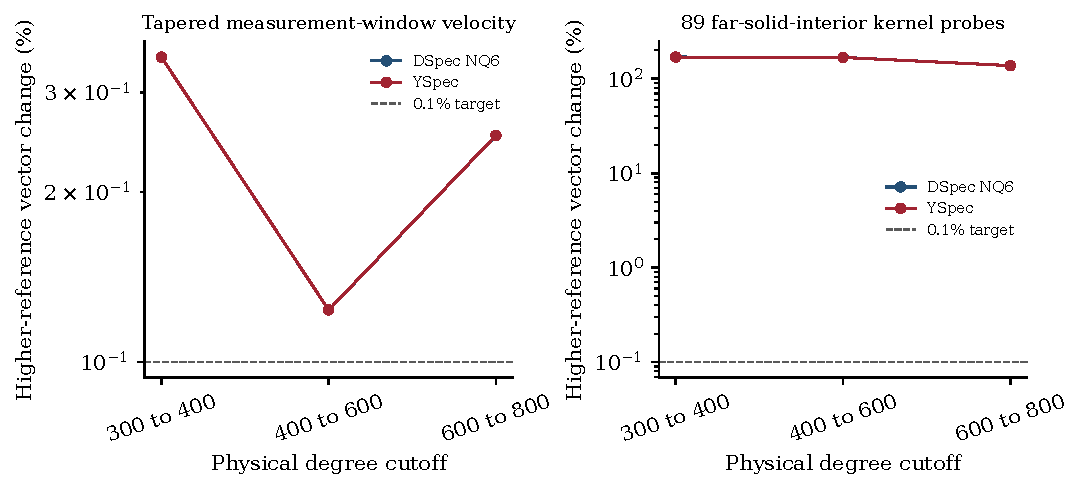
\includegraphics[width=0.95\linewidth]{figures/degree-convergence.pdf}
\caption{Observed higher-reference changes. The DSpec NQ6 radial control fails at L800, so its changes are not a pure angular-error estimate. YSpec independently exhibits the same large cutoff dependence. The dashed line is the 0.1\% operational target.}
\end{figure}
\begin{figure}[H]\centering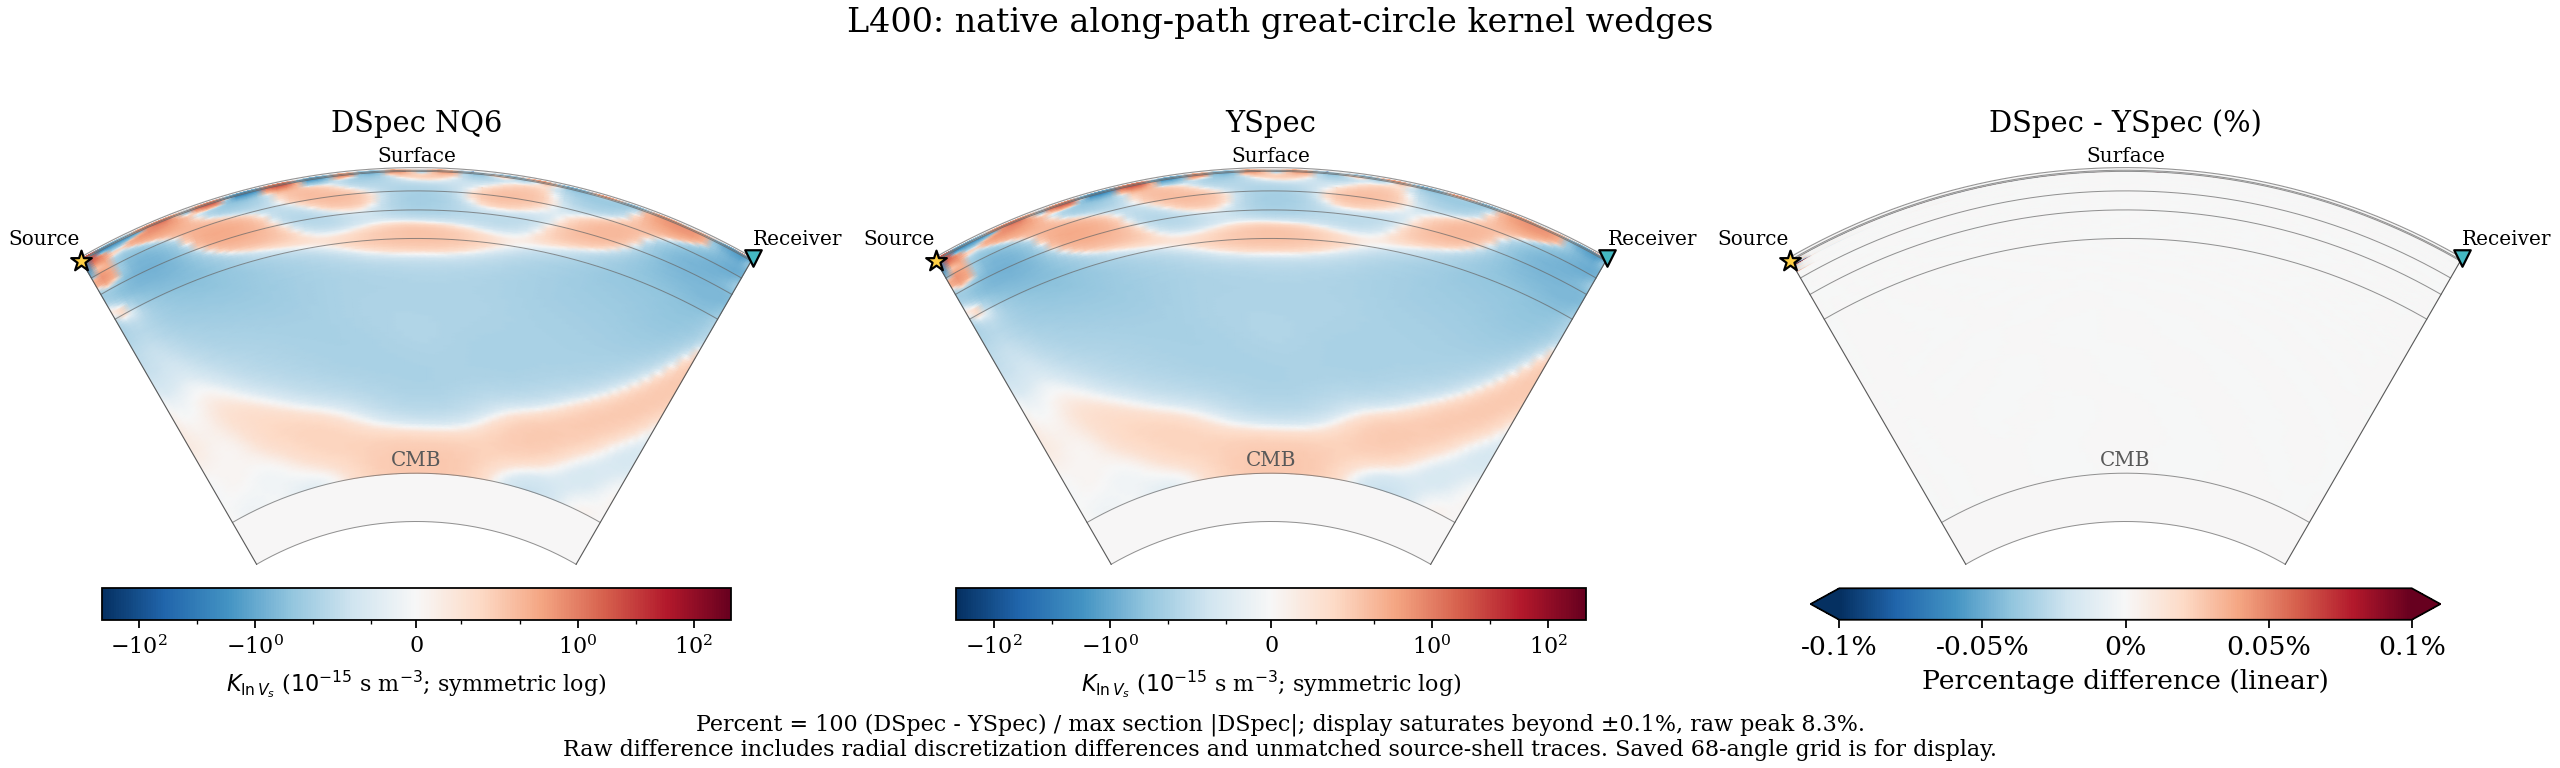
\includegraphics[width=\linewidth]{figures/kernel-comparison-L400.png}
\caption{L400: DSpec, YSpec and linear percentage difference. Physical kernel panels share the symmetric-log scale; percentage colours saturate at $\pm0.1\%$, with raw peak 8.30\%.}
\end{figure}
\begin{figure}[H]\centering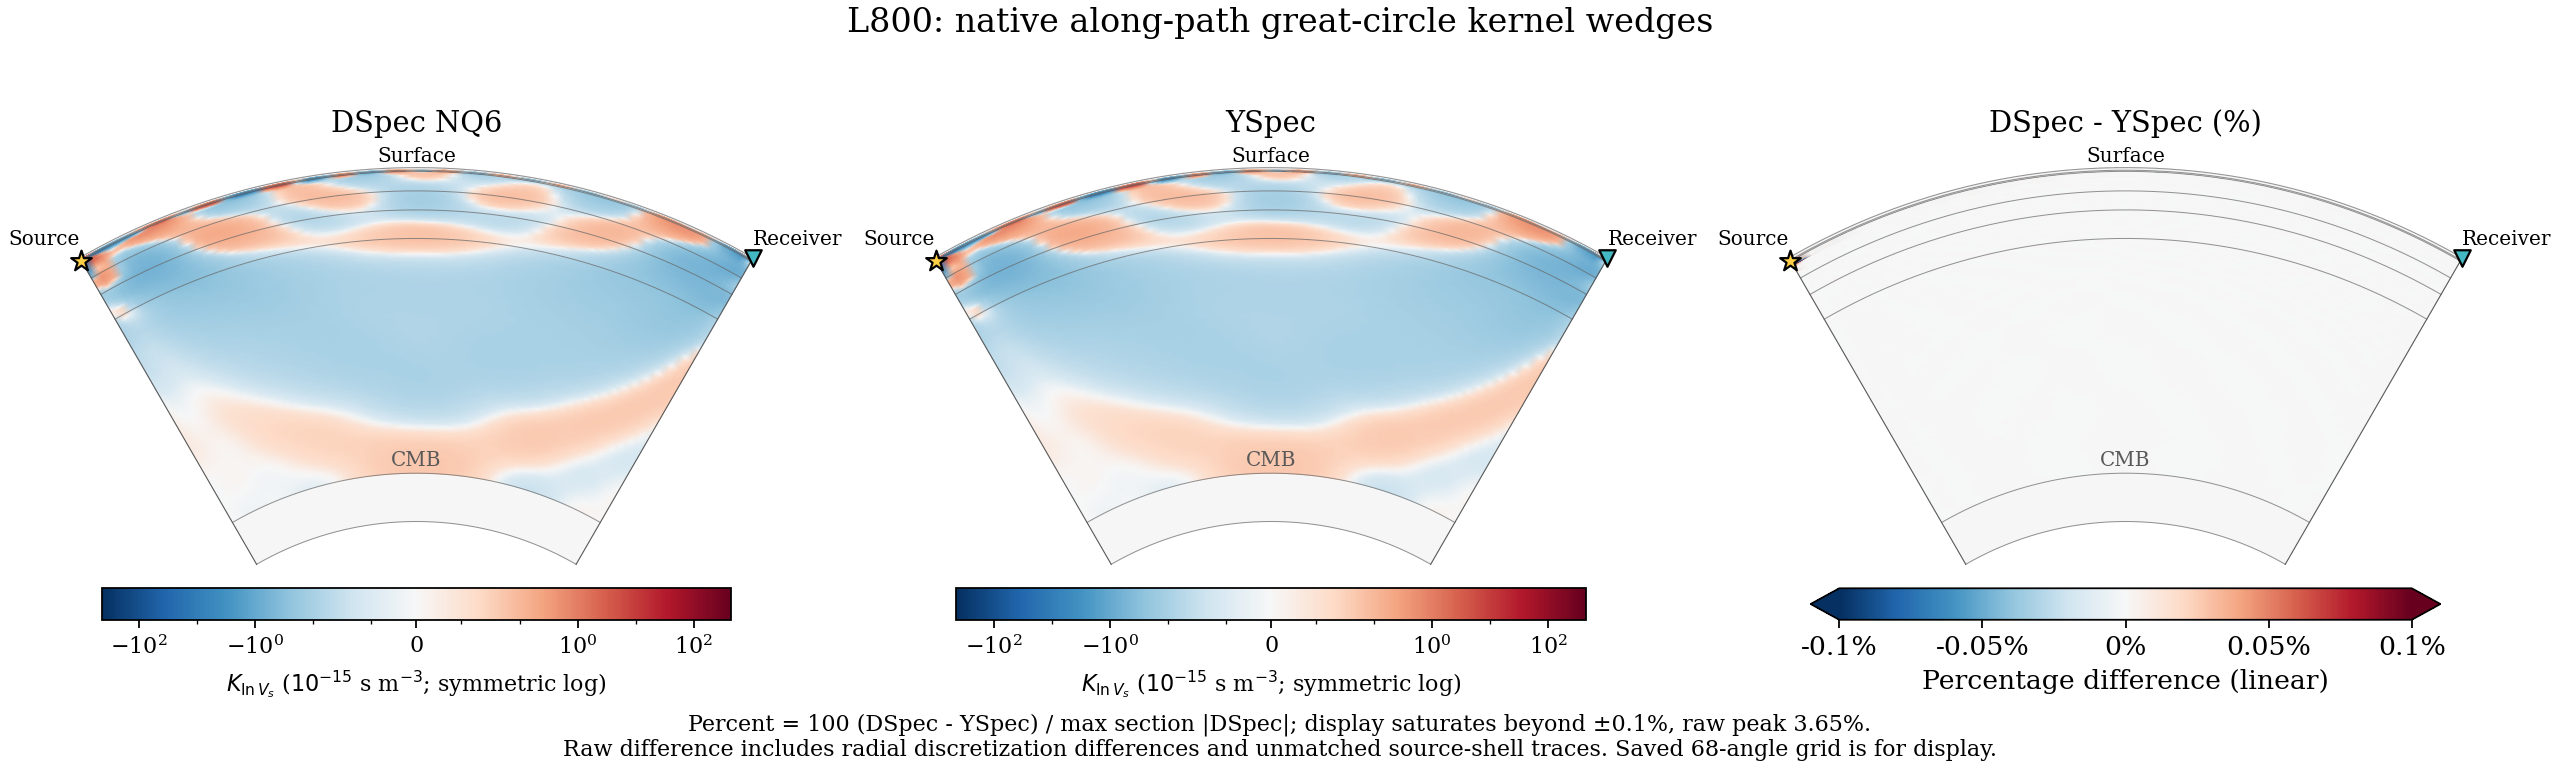
\includegraphics[width=\linewidth]{figures/kernel-comparison-L800.png}
\caption{L800: the same scales and conventions. Raw percentage peak is 3.65\%. Displayed differences include radial error and unmatched source-shell traces; these section extrema differ from the required 89-probe norm. The coarse saved angles do not resolve high-L spatial bandwidth.}
\end{figure}

\newpage
\section{Radial accuracy must be revisited at higher degree}
All angular-ladder DSpec cases use NQ6 and a fixed normalized mesh parameter. Its value is $h=0.02035382429229197$; it is not a length in metres. L800 was repeated at NQ8 and NQ10 with exactly the same element boundaries.
\begin{center}\small\begin{tabular}{lrrr}\toprule
L800 change & Window $u$ (\%) & Far kernel (\%) & Worst depth metric (\%)\\\midrule
NQ6 to NQ8 & 0.000122 & 0.759479 & 2.293048 \\
NQ6 to NQ10 & 0.000064 & 0.787197 & 2.112261 \\
NQ8 to NQ10 & 0.000060 & 0.038370 & 0.187392 \\
\bottomrule\end{tabular}\end{center}
The last column is the maximum over each required depth cohort's relative vector norm and maximum absolute difference divided by that cohort's reference maximum. All three comparisons fail the complete criterion. NQ8 versus NQ10 passes the aggregate far-vector test (0.038370\%) but fails the 50 km depth stratum: vector change 0.187392\%, maximum-scaled change 0.185817\%. An aggregate norm alone would hide that failure.

Thus the radial stability established at L200 did not transfer to NQ6 at L800. This does not establish that NQ10 itself is inaccurate; agreement with a lower order is not an exact error estimate.

\section{Cross-code agreement and its limits}
\begin{center}\small\begin{tabular}{lrr}\toprule
Matched calculation & Window $u$ (\%) & Far kernel (\%)\\\midrule
L400, NQ6 & 0.000102 & 0.105884 \\
L600, NQ6 & 0.000111 & 0.632812 \\
L800, NQ6 & 0.000093 & 0.788058 \\
\bottomrule\end{tabular}\end{center}
These differences use YSpec as reference and each code's own measurement weights. The earlier close NQ6 agreement at L100--L300 must not be extrapolated to higher cutoffs. The L800 kernel comparison improves strongly with radial polynomial order:
\begin{center}\small\begin{tabular}{lr}\toprule
DSpec order versus YSpec at L800 & Far kernel difference (\%)\\\midrule
NQ6 & 0.788058 \\
NQ8 & 0.038709 \\
NQ10 & 0.001043 \\
\bottomrule\end{tabular}\end{center}
NQ10 agrees with YSpec very closely on this vector. That is encouraging evidence about radial accuracy at fixed L800; it does not establish angular convergence, or replace the predeclared depth-by-depth self-convergence checks. YSpec's SEM-like output mesh is sampling only, not its ODE-solver discretization; its ODE tolerance remains $10^{-7}$.

\newpage
\section{Where the kernel still changes}
The L600-to-L800 DSpec NQ6 kernel change is not confined to exact source-shell samples:
\begin{center}\small\begin{tabular}{rrrr}\toprule
Depth (km) & Probe count & Vector change (\%) & Max-scaled change (\%)\\\midrule
10 & 10 & 129.049967 & 129.263742 \\
24 & 10 & 134.471693 & 136.918872 \\
29 & 10 & 136.216733 & 139.086463 \\
30 & 10 & 140.536384 & 138.686023 \\
50 & 10 & 130.106817 & 127.065249 \\
100 & 11 & 6.327292 & 7.588112 \\
300 & 14 & 0.184276 & 0.188970 \\
500 & 14 & 0.212822 & 0.216538 \\
\bottomrule\end{tabular}\end{center}
The shallow groups are especially unstable, but even the 300 and 500 km groups exceed 0.1\%. Exact source-shell traces and material-interface/near-contact cohorts are retained separately as diagnostics; they are not required bounded-pointwise convergence tests.

Holding the L800 adjoint weights fixed changes the far-vector L600-to-L800 result only from 137.884259\% to 137.835946\%. The large observed difference therefore cannot be explained simply by the small change in waveform-derived weighting. The counterfactual is explicitly $P_{800}C_L$; it is not a native lower-cutoff kernel or an independent YSpec unit-field calculation. Products include cross terms, so their cutoff differences are not additive isolated-degree kernel contributions.

All saved native sections are finite. This establishes neither a bounded point-source/receiver limit nor divergence. No new $H^1$ formulation, regularization, smoothing, receiver averaging or contact correction was introduced. The current API does not support an independent high-L three-dimensional action validation within the bounded study; that gap was documented before results. Study 1's low-degree finite-difference action test retains only its original scope.

\section{Acceptance and stopping point}
Before results, acceptance required the chosen cutoff versus L800 and two successive increments to pass 0.1\% for the tapered waveform, $N$, $P$, and every required kernel-cohort vector/max-scaled measure. Zero reference cases are explicit, with no arbitrary denominator floors. DSpec additionally required the L800 radial controls to pass. YSpec's angular result is reported separately.

No candidate passed. L600 also has only one higher increment, and L800 has no higher reference. The conditional two-job NQ10 extension required \emph{all} NQ8-to-NQ10 radial measures to pass; its trigger failed, so no extra jobs were run. No calculation above L800 was started.

The next scientific stage should first secure a radial reference at L800 by modest $h$ refinement or higher order, then investigate frequency-resolved high-degree field tails and their shallow spatial behavior before selecting a further angular ladder. That is a proposal, not executed work. Changing the frequency filter or measurement window requires its own convergence check.

\newpage
\section{Execution, memory coordination and evidence}
Eight sequential physical jobs completed with unchanged declared inputs, verified cleanup, and 132 data outputs plus eight logs hash-checked. The finalized producer snapshot begins \texttt{35ac18a3}; the separately supervised checker returned zero with all 241 inputs unchanged and cleanup verified. Its report begins \texttt{c9a162ad}; operational success is distinct from its failed accuracy criteria.

The scientific source changes were limited to the isolated bounded high-degree controls, explicit workspace policy and metadata. The radial/modal/angular mathematics were retained. One frozen native binary was built on Tunya; its SHA-256 begins \texttt{d7ffb6cb}. Luna high implemented and Sol 6.1 high reviewed the plan, source, build, input closures, operators, executed evidence and numerical findings independently.

The user requested a combined active-memory ceiling of 900 GB on Tunya. Coordination with CCDSM and DSpecM3D Implementation preserved Pilot's separate 8 GB reservation and the existing CCDSM limits, and admitted DSpecM1D to its own 40 GB/12-task/zero-swap/eight-core slice. One 32 GiB build, 16 GiB numerical campaign or 8 GiB checker ran at a time. All descendants were inside kernel-owned services; the original identity-aware user-space supervisor also remained active.

The same shared active-RAM guardian was extended only to discover the new slice/prefix. Its active-memory definition excludes reclaimable Linux memory and reported evictable ARC, with protective thresholds at 825/875 GB below the 900 GB boundary. The guardian's preserved old epoch is distinct from its new observed-peak epoch. The maximum numerical resident memory observed by the user-space supervisor was 6.7937 GiB; this is not kernel aggregate accounting or a machine-wide kernel memory cap.

At completion, all three DSpecM1D services were inactive and our slice contained zero tasks. Its kernel-accounted peak was 7.287 GB, with zero memory-limit or OOM events. Shared active RAM was 81.949 GB and its peak observed in the new guardian epoch was 90.397 GB. These are sampled active-memory estimates under the stated definition, not cache-inclusive occupancy. CCDSM and DSpecM3D Implementation were notified to release our logical 40 GB reservation; their other work and guardian were left running.

The staging checks initially caught two incorrectly declared external build paths and stopped before numerical execution. The old plans/packages and stopped attempt were preserved; a reviewed recovery added the corrected terminal plan without overwriting the original. Local retrieval-path/receipt-writer failures were also retained. No scientific calculation was repeated to repair metadata or retrieval.

Figures are reproducible from hash-bound raw files. The saved wedges have 68 along-path and 10 cross-path angles, separately from the solved L; interpolation is for display and does not resolve the full high-L angular bandwidth. Linear percentage difference panels use the full displayed DSpec-section maximum, whereas the tables use the named cohort norms/maxima. Display saturation and unmatched source-shell traces are labelled.

All changes/results remain isolated. No production integration, new optimization, broader band/window campaign or unapproved high-degree extension followed.

\medskip\noindent\small Full hashes and supporting source are retained in \texttt{reports/report-data.json}, the delivery manifest, the independent AFTER-results review, and the producer/checker raw evidence directories. Scientific conclusions apply only to the stated fixture and sampled quantities.
\end{document}
